\section{Theory of Liquids (Statistical Associating Fluid Theory)}
\subsection*{What is a liquid?}
\begin{frame}
  \frametitle{What is a liquid?}
  \framesubtitle{Elementary school definition}
  \begin{center}
    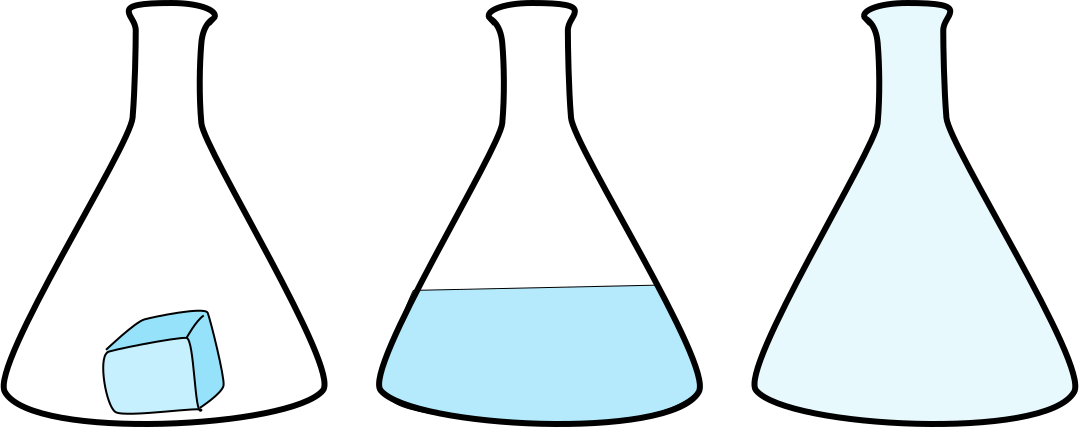
\includegraphics[width=7cm]{figs/solid-liquid-gas}
  \end{center}
  \begin{description}
  \item[Solid] Does not take the shape of its container
  \item[Liquid] Takes the shape of a container, but doesn't fill it
  \item[Gas] Takes the shape of its container and fills it
  \end{description}
\end{frame}

\begin{frame}
  \frametitle{What is a liquid?}
  %\framesubtitle{Phase diagram}
  \begin{center}
    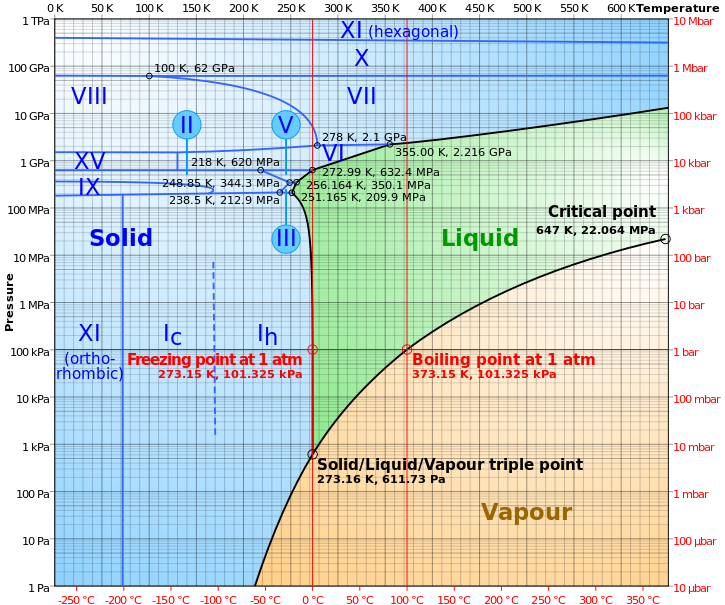
\includegraphics[height=7.8cm]{figs/water-phase-diagram}
  \end{center}
\end{frame}

\begin{frame}
  \frametitle{What is a liquid?}
  \framesubtitle{Energy versus entropy}
  \begin{center}
    \includegraphics<1>[width=7cm]{figs/energy-solid}
    \includegraphics<2>[width=7cm]{figs/energy-solid-gas}
    \includegraphics<3->[width=7cm]{figs/energy-solid-gas-liquid}
  \end{center}
  \begin{description}
  \item[Solid] Energy dominates, entropy is a small perturbation
  \item<3->[Liquid] Energy and entropy are balanced
  \item<2->[Gas] Entropy dominates, energy is a small perturbation
  \end{description}
  \begin{block}{Perturbation theory}<4->
    \begin{itemize}
    \item An ``easy'' problem we know how to solve
    \item A ``hard'' correction that is small
    \item We construct a power series to solve combined problem
    \end{itemize}
  \end{block}
  %% \begin{enumerate}
  %% \item Solid and gas perturbation expansion
  %% \item No easy perturbation for liquid
  %% \item Ice floats
  %% \item Critical point
  %% \item Below the triple point
  %% \end{enumerate}
\end{frame}

%% \section[SAFT]{Understanding water using Statistical Associating
%%   Fluid Theory}

%% \subsection*{Simple liquids}
%% \begin{frame}
%%   \frametitle{Dense fluids}
%%   In order to use a perturbative approach, we need a ``solved''
%%   problem that is similar to a liquid.

%%   \begin{block}{Correlation function}<2->
%%     \vspace{-3em}
%%     \hfill \includegraphics[width=5cm, angle=270]{figs/correlation}\\
%%     %\vspace{-1em}
%%     \hfill\mycite{Soper}{J. Chem. Phys.}{2000}\\
%%     The correlation function $g(r)$ tells us how likely we are to find
%%     an atom at a given distance from any other atom.
%%   \end{block}
%% \end{frame}

\begin{frame}
  \frametitle{Dense fluids (Hard spheres)}
  In order to use a perturbative approach, we need a ``solved''
  problem that is similar to a liquid.
  \begin{block}{Hard-sphere fluid}
    \begin{itemize}
    \item Captures the repulsive portion of the structure
    \item All entropy, no energy!
    \item Not actually a liquid
    \end{itemize}
    \begin{center}
      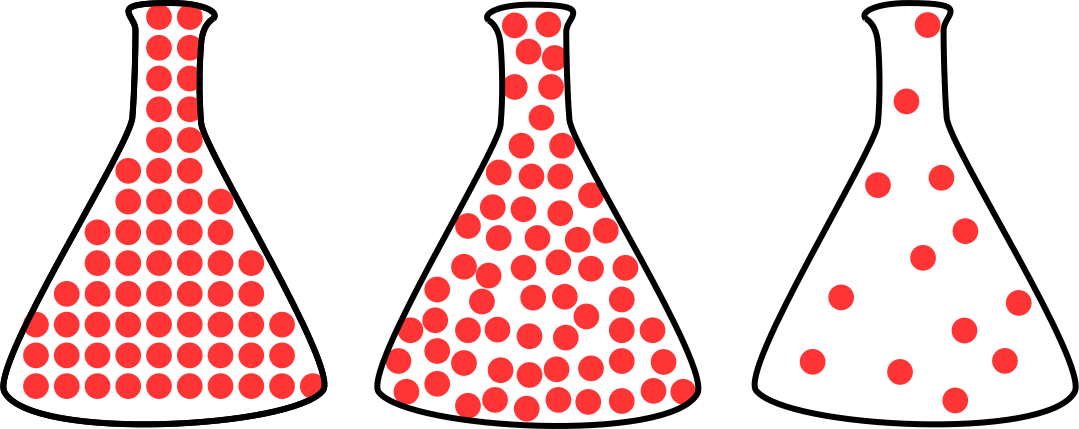
\includegraphics[width=8cm]{figs/hard-spheres}
    \end{center}
  \end{block}
\end{frame}

\begin{frame}
  \frametitle{Simple liquids (adding dispersion interaction)}
  \begin{itemize}
  \item Perturbative attraction added to hard spheres
  \item ``High T expansion''
    \[
    F_\text{disp} = N\left(a_1(n) + a_2(n)\beta + \mathcal{O}(\beta^2)\right),
    \quad \quad \beta \equiv \frac{1}{k_BT}
    \]

    \vspace{1em} The temperature-independent $a_1$ term corresponds to
    a mean-field approximation, and incorporates correlations present
    in the hard-sphere fluid.
    \vspace{1em}

    The $a_2$ term incorporates---to first order---correlations due to
    the attraction itself.
  \end{itemize}
\end{frame}

%\subsection{Hydrogen bonding (Association)}
\begin{frame}
  \frametitle{Hydrogen bonds (adding association interaction)}
  \vspace{-2em}
  \hfill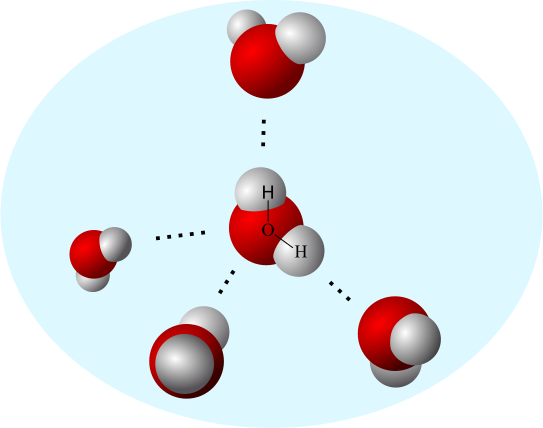
\includegraphics[width=7cm]{figs/hydrogen-bonds}\hspace{-3em}
  \vspace{-2em}
  \begin{itemize}
  \item Highly directional bonds
  \item Not a ``small'' interaction (around $4k_BT$)
  \item Small volume of interaction
  \item Wertheim's Thermodynamic Perturbation Theory\\ \hfill
    \mycite{Wertheim}{J. Stat. Phys.}{1984,1986}
  \end{itemize}
\end{frame}

\begin{frame}
  \frametitle{Putting it all together:  SAFT for water}
  All these terms combined describe SAFT, a well-established theory
  for \emph{homogeneous} liquids.
  \begin{center}
    \vspace{-1em}
    \includegraphics[height=6cm]{../../papers/water-saft/figs/pressure-with-isotherms-truncated}
  \end{center}
  \hfill Clark \emph{et al}, \emph{Mol. Phys.}
  (2006)
\end{frame}

\section{Handling interfaces}

\begin{frame}
  \frametitle{Interfaces:  Classical Density Functional Theory}
  In order to describe liquid \emph{interfaces} we need a theory that
  can handle \emph{inhomogeneous} configurations.
  \begin{block}{Classical Density Functional Theory (cDFT)}
    \[\Omega = \min_{n(\rr)} \left\{ F[n(\rr), T] + \int (V(\rr)-\mu) n(\rr)d\rr \right\}
    \]
    \begin{itemize}
    %% \item $\Omega$ is grand potential
    %% \item $n(\rr)$ is number density of atoms or molecules
    %% \item $V(\rr)$ is an arbitrary external potential energy
    %% \item $\mu$ is the chemical potential
    \item minimize the grand potential $\Omega$
    \item $F[n(\rr),T]$ is a universal functional for a given fluid
    \end{itemize}
  \end{block}
\end{frame}

\begin{frame}
  \frametitle{Testing the theory:  Monte Carlo simulation}
  \vspace{-0.8em}
  \begin{center}
    \animategraphics[height=20em]{.6}{anim/mc-slow-}{000}{30}\\
    \vspace{-2.0em}
    hard circles between two walls
  \end{center}
\end{frame}

\begin{frame}
  \frametitle{Testing the theory:  Monte Carlo simulation for $n(\rr)$}
  \vspace{-0.8em}
  \begin{center}
    \animategraphics[height=20em,autoplay]{.6}{anim/mc-density-}{000}{30}\\
    \vspace{-2.0em}
    hard circles between two walls
  \end{center}
\end{frame}

